% Use only LaTeX2e, calling the article.cls class and 12-point type.

\documentclass[12pt]{article}

% Users of the {thebibliography} environment or BibTeX should use the
% scicite.sty package, downloadable from *Science* at
% www.sciencemag.org/about/authors/prep/TeX_help/ .
% This package should properly format in-text
% reference calls and reference-list numbers.

\usepackage{scicite}
\usepackage[]{algorithm2e}
\usepackage{amsmath,amssymb}
\usepackage{bbm}

\usepackage{graphicx}
\graphicspath{ {/Users/wenxuandeng/GoogleDrive/sucksalt/group_lasso/code/GroupLasso/CodeForFigures/} }

% Use times if you have the font installed; otherwise, comment out the
% following line.

\usepackage{times}

% The preamble here sets up a lot of new/revised commands and
% environments.  It's annoying, but please do *not* try to strip these
% out into a separate .sty file (which could lead to the loss of some
% information when we convert the file to other formats).  Instead, keep
% them in the preamble of your main LaTeX source file.


% The following parameters seem to provide a reasonable page setup.

\topmargin 0.0cm
\oddsidemargin 0.2cm

\textwidth 16cm 
\textheight 21cm
\footskip 1.0cm


%The next command sets up an environment for the abstract to your paper.

\newenvironment{sciabstract}{%
\begin{quote} \bf}
{\end{quote}}


% If your reference list includes text notes as well as references,
% include the following line; otherwise, comment it out.

\renewcommand\refname{References and Notes}

% The following lines set up an environment for the last note in the
% reference list, which commonly includes acknowledgments of funding,
% help, etc.  It's intended for users of BibTeX or the {thebibliography}
% environment.  Users who are hand-coding their references at the end
% using a list environment such as {enumerate} can simply add another
% item at the end, and it will be numbered automatically.

\newcounter{lastnote}
\newenvironment{scilastnote}{%
\setcounter{lastnote}{\value{enumiv}}%
\addtocounter{lastnote}{+1}%
\begin{list}%
{\arabic{lastnote}.}
{\setlength{\leftmargin}{.22in}}
{\setlength{\labelsep}{.5em}}}
{\end{list}}


% Include your paper's title here

\title{Generalized Group Elastic Net for Predictive Biomarker Identification} 


% Place the author information here.  Please hand-code the contact
% information and notecalls; do *not* use \footnote commands.  Let the
% author contact information appear immediately below the author names
% as shown.  We would also prefer that you don't change the type-size
% settings shown here.

\author
{Wenxuan Deng$^{1}$
\\
\\
\normalsize{$^{1}$Department of Biostatistics, Yale University,}
}

% Include the date command, but leave its argument blank.

\date{}



%%%%%%%%%%%%%%%%% END OF PREAMBLE %%%%%%%%%%%%%%%%



\begin{document} 

% Double-space the manuscript.

\baselineskip24pt

% Make the title.

\maketitle 



% Place your abstract within the special {sciabstract} environment.

\begin{sciabstract}
  Predictive biomarker identification is a significant problem when targeting
  patient subpopulation who gets an enhanced benefit under treatment. This paper proposed
  a new method, Predictive Effects Net (PEN), based on group lasso and special hierarchical structure for figuring
  out predictive effects. The new approach takes predictive biomarkers as interaction effects between
  treatment and biomarker. To show PEN has an supreme performance, this paper shows simulations
  in different scenerios and comparisons with several other variable selection methods.
\end{sciabstract}



% In setting up this template for *Science* papers, we've used both
% the \section* command and the \paragraph* command for topical
% divisions.  Which you use will of course depend on the type of paper
% you're writing.  Review Articles tend to have displayed headings, for
% which \section* is more appropriate; Research Articles, when they have
% formal topical divisions at all, tend to signal them with bold text
% that runs into the paragraph, for which \paragraph* is the right
% choice.  Either way, use the asterisk (*) modifier, as shown, to
% suppress numbering.

\section*{Introduction}

Prognostic biomarkers and predictive biomarkers.

Why decision trees is not workable? Because the sample size in real clinical datasets is too small, typically no more than 100 patients.

Group lasso \cite{yuan2006model}

Elastic net \cite{zou2005regularization} adaptive weights for elastic net \cite{zou2009adaptive}

Hierarchical Group lasso for interactions \cite{lim2015learning}

Overlapping group lasso \cite{jacob2009group}\cite{percival2012theoretical}\cite{obozinski2011group}

Sparse Group Lasso \cite{friedman2010note} \cite{simon2013sparse}

Structured group lasso \cite{zhao2009composite}
Group lasso for logistic regression \cite{meier2008group}

Other variable selection methods:

GUIDE: a regression tree \cite{loh2015regression}\cite{loh2002regression}

SIS: screening \cite{fan2008sure}\cite{fan2009ultrahigh}

SIR: \cite{jiang2013sliced}\cite{li2018robust}

Stepwise selection: \cite{miller1984selection}

\section*{Methods}

\subsection*{Model}


$$Y=X_0\beta_0 + X_T\beta_\tau + X_1\beta_1 + X_T\otimes X_1 \beta_2+\epsilon$$


Where $X_0$ is the baseline variables, $X_T$ is the treatment variable, $X_1$ is the high dimensional design matrix of genes, i.e. gene expression levels, SNP and mutations, and $X_T\otimes X_1$ is the interaction between genes and treatment. $\beta=(\beta_0, \beta_\tau, \beta_1, \beta_2)$ is the corresponding coefficients. $\epsilon$ is random error.

Let $$X=[X_0,X_T,X_1^{(1)},\dots,X_m^{(1)},X_TX_1^{(1)},\dots,X_TX_1^{(m)}]$$ and $$\beta=[\beta_0,\beta_\tau,\beta_1^{(1)},\dots,\beta_1^{(m)},\beta_2^{(1)},\dots,\beta_2^{(m)}]$$ For each gene $l$, its prognostic and predictive design matrix is denoted as $X^{(l)}=[X_1^{(l)},X_2^{(l)}]$ where $X_2^{(l)}=X_TX_1^{(l)}$ and its corresponding coefficients are $\beta^{(l)}=[\beta_1^{(l)},\beta_2^{(l)}]$

\subsection*{Loss Function}

We used group lasso and elastic net for variables selection when $n\ll p$, and assumed the hierarchical relationship between prognostic biomarkers and predictive biomarkers, that is the predictive biomarkers should be a prognostic biomarkers. The loss function is 

$$\min_{\beta} f(\beta|Y,X_0,X_T,X_1) + g(\beta)$$

$$g(\beta)=\lambda_1\sum_i\phi_i|\beta_2^{(i)}|+\lambda_1\sum_i\psi_i\sqrt{(\beta_1^{(1)})^2+(\beta_2^{(1)})^2}+\lambda_2(\parallel\beta_1\parallel_2^2+\parallel\beta_2\parallel_2^2)$$

Where $\beta=(\beta_0,\beta_\tau,\beta_1,\beta_2)$ is the parameter, and $f(\beta|Y,X_0,X_T,X_1) $ is $L$-2 loss function. When the model is the ordinary linear model, the $L$-2 loss function is $\parallel Y-(X_0\beta_0 + X_T\beta_\tau + X_1\beta_1+ X_T\otimes X_1 \beta_2) \parallel^2$. Penalty function $g(\beta)$ can construct a complex hierarchical selection of $\beta_1$ and $\beta_2$, that nonzero $\beta_2$ is a sufficient but not necessary condition for nonzero $\beta_1$. The contour plot for a pair of $\beta_1$ and $\beta_2$ is shown in Figure 1. $\lambda_1$ and $\lambda_2$ are regularization parameters.

\begin{figure}[t]
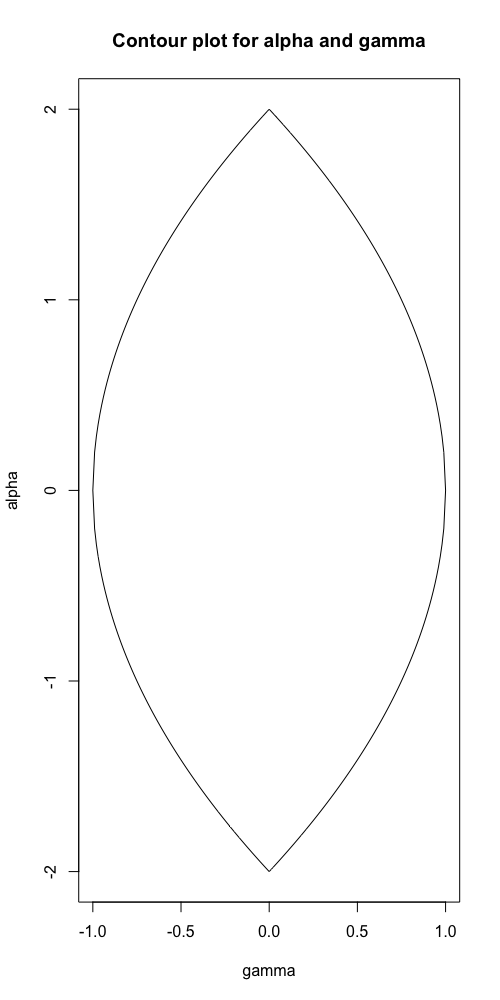
\includegraphics[scale=0.5]{Contour.png}
\centering
\end{figure}


\subsection*{Criterion and Adaptive Weights} 

\subsubsection*{KKT conditions}

KKT \cite{tibshirani2013lasso}

For group $\hat{\beta}^{(l)}$, the KKT condition is 

\begin{equation} \label{KKT}
  \begin{split}
  {X^{(l)}}^T(Y-X^T\hat{\beta}) &= \lambda_1\phi_l \begin{bmatrix}
         0 \\
         v 
       \end{bmatrix}
       + \lambda_1\psi_lu+\frac{1}{2}\lambda_2\hat{\beta}^{(l)}
  \end{split}
\end{equation}

where

\begin{align}
v & = \begin{cases}
  \text{sign}(\hat{\beta}_2^{(l)}) & \text{ \qquad  if $\hat{\beta_2}^{(l)}\neq 0$} \\
  \in\{v:|v|_1\leq 1\}&  \text{ \qquad  if $\hat{\beta_2}^{(l)}= 0$} 
\end{cases}
\\
u & = \begin{cases} 
  \hat{\beta}^{(l)}/\parallel \hat{\beta}^{(l)} \parallel_2 & 
  \text{ \qquad  if $\hat{\beta}^{(l)}\neq 0$} \\
  \in \{u:\parallel u\parallel_2\leq 1\} & \text{\qquad if $\hat{\beta}^{(l)}= 0$}
\end{cases} 
\end{align}

\begin{itemize}
\item We now investigate when $\hat{\beta}^{(l)}=0$ satisfies KKT condition \ref{KKT}. We propose the following condition
\begin{equation} \label{zero}
  \begin{split}
S(  {X_1^{(l)}}^T  r_{(-l)},0)^2+S(  {X_2^{(l)} }^T  r_{(-l)},\lambda_1\phi_l)^2\leq \lambda_1^2\psi_l^2
\end{split}
\end{equation}
where 

\begin{align}
S(z,a)=\text{sign}(z)(|z|-a)_+
\end{align}
and 

\begin{align}
r_{(-l)}=Y- {X^{(-l)}}^T  \hat{\beta}^{(-l)}
\end{align}

Under this condition, we can find 
\begin{align}
  u & = \begin{bmatrix}
    \frac{X_1^{(l)}r_{(-l)}}{\lambda_1\psi_l} \\
    \frac{S(  {X_2^{(l)} }^T r_{(-l)},\lambda_1\phi_l)}{\lambda_1\psi_l}
  \end{bmatrix}
  \\
  v & = \begin{bmatrix}
    0 \\
    \frac{  {X^{(l)}}^T  r_{(-l)}-S( {X_2^{(-l)}}^T r_{(-l)},\lambda_1\phi_l)}{\lambda_1\psi_l}
  \end{bmatrix}
\end{align}

such that $\parallel u\parallel_2\leq 1$ and $|v|_{\infty}\leq 1$. By simple algebra, the subgradient equation \ref{KKT}
was satisfied with $\hat{\beta}^{(l)}=0$

\item if KKT condition holds with $\hat{\beta}^{(l)}\neq 0$ but $\hat{\beta}_2^{(l)} = 0 $, the KKT condition can be reformulated as following 
\begin{align}
  {X^{(l)}}^T(Y- {X^{(-I(l))}}^T \hat{\beta}^{(-I(l))})=\lambda_1\phi_l \begin{bmatrix}
    0 \\
    v 
  \end{bmatrix}
  + \lambda_1\psi_l \frac{\hat{\beta}^{(l)}}{\parallel \hat{\beta}^{(l)} \parallel_2 } +\frac{1}{2}\lambda_2\hat{\beta}^{(l)}
\end{align}

To satisfy $\hat{\beta}_2^{(l)}=0$ and KKT condtion, we should have
\begin{align}
 {X_2^{(l)}}^T r_{(-I(l))}\leq \lambda_1\phi_l  
\end{align}
where $r_{(-I(l))}=Y- {X^{(-I(l))}}^T \hat{\beta}^{(-I(l))}$ and $I(l)$ is the interaction effect
nested in biomarker $l$th group.


\item if KKT condition holds with $\hat{\beta}^{(l)}\neq 0$ as well as $\hat{\beta}_2^{(l)}\neq 0$, the KKT condition is reformulated as

\begin{align}
  {X^{(l)}}^T(Y-  {X^{(-I(l))}}^T \hat{\beta}^{(-I(l))})=\lambda_1\phi_l \begin{bmatrix}
    0 \\
    \text{sign}(\hat{\beta}_2^{(l)})
  \end{bmatrix}
  + \lambda_1\psi_l \frac{\hat{\beta}^{(l)}}{\parallel \hat{\beta}^{(l)} \parallel_2 } +\frac{1}{2}\lambda_2\hat{\beta}^{(l)}
\end{align}

Then we get

\begin{equation} 
  \begin{split}
  \hat{\beta}_2^{(l)} & =\frac{ {X_2^{(l)}}^T (Y-X^T\hat{\beta}^{(-I(l))})-\lambda_1\phi_l\text{sign}(\hat{\beta}_2^{(l)})}{{X_2^{(l)}}^TX_2^{(l)}+\frac{\lambda_1\psi_l}{\parallel \hat{\beta}^{(l)} \parallel_2} + \frac{1}{2}\lambda_2} \\
  & = \frac{ S( {X_2^{(l)}}^Tr_{(-I(l))}, \lambda_1\phi_l ) }{ {X_2^{(l)}}^TX_2^{(l)}+\frac{\lambda_1\psi_l}{\parallel \hat{\beta}^{(l)} \parallel_2} + \frac{1}{2}\lambda_2 } 
\end{split}
\end{equation}
  
  \begin{equation} 
    \begin{split}
  \hat{\beta}_1^{(l)} & =  \frac{ {X_2^{(l)}}^T r_{(-G(l))} }{ {X_1^{(l)}}^TX_1^{(l)}+\frac{\lambda_1\psi_l}{\parallel \hat{\beta}^{(l)} \parallel_2} + \frac{1}{2}\lambda_2 } 
\end{split}
\end{equation}
  
  \begin{equation} 
    \begin{split}
  \hat{\beta}_0 & = \frac{ X_0^T r_{(-0)} }{ X_0^TX_0 } 
\end{split}
\end{equation}
  
  \begin{equation} 
    \begin{split}
  \hat{\beta}_{\tau} & = \frac{ X_T^T r_{(-T)} }{ X_T^TX_T }
\end{split}
\end{equation}

\end{itemize}

\subsubsection*{Adaptive Weights}

To give each biomarker equal probability to be prognostic and predictive,
we define adaptive weights via a null model that the residual $\epsilon=r_{(-I(l))}$ 
is a normal random error where $\epsilon\sim N(0,\sigma^2)$ when $\hat{\beta}_2^{(l)}=0$.
Let
\begin{equation} \label{phil}
  \begin{split}
  \parallel {X_2^{(l)}}^T r_{(-I(l))} \parallel_2 & = \lambda_1\phi_l \\
  E[( {X_2^{(l)}}^T r_{(-I(l))})^2] & = \lambda_1^2\phi_l^2
\end{split}
\end{equation}
Thus, we can get $\lambda_1^2\phi_l^2 = \text{Var}( {X_2^{(l)}}^T r_{(-I(l))})$ and 

\begin{align}
  \phi_l & \propto \parallel X_2^{(l)} \parallel_2 
\end{align}

Since $\lambda_1$ is regularization parameter, we define $\phi_l=\parallel X_2^{(l)} \parallel_2$
without loss generality.

On the other hand, based on inequality \ref{zero} and results from formula \ref{phil}, we let
\begin{align}
  \mathbb{E} [ S( {X_1^{(l)}}^T r_{(-l)},0)^2+S( {X_2^{(l)}}^T r_{(-l)},\lambda_1\phi_l)^2  ] = \lambda_1^2\psi_l^2
\end{align}
and assume $ r_{(-l)} = \epsilon  \sim N(0,\sigma^2)$ if $\beta^{(l)}=0$, thus $\epsilon_1= {X_2^{(l)}}^T r_{(-l)} \sim N(0,\lambda_1^2\phi_l^2)$ and 
$\epsilon_0=\epsilon_1/\lambda_1\phi_l\sim N(0,1)$.



\begin{equation} \label{equ_1}
  \begin{split}
 \mathbb{E}[S( {X_2^{(l)}}^T r_{(-l)},\lambda_1\phi_l)^2] &  =  \mathbb{E}[\parallel \epsilon_1 \parallel_2^2 \mathbbm{1}_{|\epsilon_1|>\lambda_1\phi_l}]-2\lambda_1\phi_l\mathbb{E}[|\epsilon_1|\mathbbm{1}_{|\epsilon_1|>\lambda_1\phi_l}]  \\
  &  + \lambda_1^2\phi_l^2\mathbb{E}[\mathbbm{1}_{|\epsilon_1|>\lambda_1\phi_l}] \\
\end{split}
\end{equation}
  
  \begin{equation} \label{equ_2}
    \begin{split}
  \mathbb{E}[\parallel \epsilon_1 \parallel_2^2 \mathbbm{1}_{|\epsilon_1|>\lambda_1\phi_l}] & = 
  \mathbb{E}[\parallel \epsilon_1 \parallel_2^2 (1-  \mathbbm{1}_{|\epsilon_1|\leq\lambda_1\phi_l})] \\
  & = \lambda_1\phi_l^2(1- \mathbb{E}[ \parallel \epsilon_0 \parallel_2^2 ] \mathbbm{1}_{|\epsilon_0|\leq 1}  ) \\
  & \approx \lambda_1\phi_l^2(1- ( 0.68- 2 \frac{1}{\sqrt{2\pi}} \exp{(-0.5)} )  ) \\
  & = (0.32 +\sqrt{\frac{2}{\pi}}\exp(-0.5) ) \lambda_1^2\phi_l^2 \\
\end{split}
\end{equation}
  
  \begin{equation} \label{equ_3}
    \begin{split}
  \mathbb{E}[|\epsilon_1|\mathbbm{1}_{|\epsilon_1|>\lambda_1\phi_l}] & = \lambda_1\phi_l \mathbb{E}[|\epsilon_0|\mathbbm{1}_{|\epsilon_0|>1}]  \\
  & = \lambda_1\phi_l (\mathbb{E}|\epsilon_0| - \mathbb{E}|\epsilon_0| \mathbbm{1}_{|\epsilon_0|\leq 1} ) \\
  & =  \lambda_1\phi_l( \sqrt{\frac{2}{\pi}} - \sqrt{\frac{2}{\pi}} (1-\exp{(-0.5)}) )    \\ 
  & = \sqrt{\frac{2}{\pi}}\exp(-0.5) \lambda_1\phi_l \\
\end{split}
\end{equation}
  
  \begin{equation} \label{equ_4}
    \begin{split}
  \mathbb{E}[\mathbbm{1}_{|\epsilon_1|>\lambda_1\phi_l}] & = \mathbb{P}(|\epsilon_0|>1) \approx 0.32 
  \end{split}
\end{equation}

Take equations \ref{equ_2} - \ref{equ_4} to equation \ref{equ_1}, we can get

\begin{equation} \label{equ_5}
  \begin{split}
    \mathbb{E}[S( {X_2^{(l)}}^2 r_{(-l)},\lambda_1\phi_l)^2] &  \approx (0.64- \sqrt{\frac{2}{\pi}}\exp(-0.5) ) \lambda_1^2\phi_l^2
  \end{split}
\end{equation}

Insert results of equation (23) into (18), we define

\begin{equation}
  \begin{split}
\psi_l = \sqrt{\parallel X_1^{(l)} \parallel_2 + \{0.64 - \sqrt{\frac{2}{\pi}}\exp(-0.5) \} \parallel X_2^{(l)} \parallel_2} 
\end{split}
\end{equation}

such that
\begin{equation}
  \begin{split}
    \lambda_1^2\psi_l^2 = \lambda_1^2  [ \parallel X_1^{(l)} \parallel_2 + \{0.64 - \sqrt{\frac{2}{\pi}}\exp(-0.5) \} \parallel X_2^{(l)} \parallel_2 ]
  \end{split}
\end{equation}


\subsection*{Algorithms}

Fast iterative shrinkage-thresholding algorithm with backtracking \cite{beck2009fast}

Proximal operator for group lasso \cite{liu2010fast}

Adaptive restart for rippling behavior \cite{o2015adaptive}

Adaptive stepwise of cyclic Barzilai-Borwein spectral approach \cite{wright2009sparse}




\begin{algorithm}[H]
  initialization $\theta_0=0$ or warm start from previous run, $\tau_0=0.1$, stepsize $\eta=0.5$\;
  \While{$i\le k$}{
  $u_{i}=\theta_{i-1}-\tau_i \bigtriangledown f(\theta_{i-1})$
 Find the smallest nonnegative integers $s_i$ such that with $\tau_{i}=\eta^{s_{i-1}}\tau_{i-1}$, $(f+g)(P_{\tau_i,g}(u_i))\le  Q_{\tau_i,g}(P_{\tau_i,g}(u_i),u_i)$\;
 Then, we compute $t_{i}=P_{\tau_i,g}(u_i)$
 And accelarate the computation by setting 
 \eIf{$f(\theta_{i}+g(\theta_i))>f(\theta_{i-1})+g(\theta_{i-1})$}{  $\rho_i=1$
    }{
    $\rho_i=\frac{1+\sqrt{1+4\rho_{i-1}^2}}{2}$
   }
   $\theta_i=t_i+(\frac{\rho_{i-1}-1}{\rho_i})(t_i-t_{i-1})$ and find $\tau_{i+1}$ that $\tau_{i+1}I$ can mimic the Hessian $ \bigtriangledown^2f(\theta_i)$
  }
  \caption{Patient Subgroup Identification Group Lasso Algorithm}
 \end{algorithm}
 

\subsection*{Experiments}

Signal to noise ratio: $SNR=\frac{Var(X\beta)}{Var(\epsilon)}$


\subsection*{Future Steps}

check KKT condition

% Your references go at the end of the main text, and before the
% figures.  For this document we've used BibTeX, the .bib file
% scibib.bib, and the .bst file Science.bst.  The package scicite.sty
% was included to format the reference numbers according to *Science*
% style.


% \bibliography{scibib}

%  te\bibliographystyle{Science}

\bibliographystyle{unsrt}
\bibliography{scibib}



% Following is a new environment, {scilastnote}, that's defined in the
% preamble and that allows authors to add a reference at the end of the
% list that's not signaled in the text; such references are used in
% *Science* for acknowledgments of funding, help, etc.






% For your review copy (i.e., the file you initially send in for
% evaluation), you can use the {figure} environment and the
% \includegraphics command to stream your figures into the text, placing
% all figures at the end.  For the final, revised manuscript for
% acceptance and production, however, PostScript or other graphics
% should not be streamed into your compliled file.  Instead, set
% captions as simple paragraphs (with a \noindent tag), setting them
% off from the rest of the text with a \clearpage as shown  below, and
% submit figures as separate files according to the Art Department's
% instructions.


\clearpage





\end{document}




















